\section{Sampling methods}
\begin{itemize}
	\item In the previous chapter, we have seen that we can perform inference by approximating the posterior distribution. However, as alternative, we can also consider Monte Carlo techniques, i.e. sampling
	\item In most practical cases, we often want to evaluate expectations over the posterior. This we can approximate by an average over samples:
	$$\E_{p(\bm{x})}\left[f(\bm{x})\right] \approx \frac{1}{N}\sum_{n=1}^{N} f(\bm{x}_n), \hspace{2mm} \bm{x}_n\sim p(\bm{x})$$
	This can be for example used for prediction:
	$$p(y^{*}|x^{*}) = \int p(y^{*}\vert x^{*}, \bm{\theta})p(\bm{\theta}|\bm{X}, \bm{Y})d\bm{\theta} = \E_{p(\bm{\theta}|\bm{X}, \bm{Y})}\left[p(y^{*}\vert x^{*}, \bm{\theta})\right] \approx \frac{1}{K}\sum_{k=1}^{K} p(y^{*}\vert x^{*}, \bm{\theta}^{(k)}), \hspace{2mm} \bm{\theta}^{(k)}\sim p(\bm{\theta}|\bm{X}, \bm{Y})$$
	\item Hence, we will look at different techniques for sampling from more complex distributions than standard Gaussians
\end{itemize}
\subsection{Regular Sampling}
\begin{itemize}
	\item As an introduction, we look at how we can sample from simple, known distributions, and verify the correctness of the Monte Carlo approximation
	\item Assume we draw $N$ samples from $p(z)$: $z_i\sim p(z)$, $i=1,...,N$
	\item We can calculate $\E\left[f\right]\approx \widehat{E\left[f\right]}=\left<f\right> = \frac{1}{N}\sum_{n=1}^{N}f(z_i)$ for approximating the expectation. Note that we introduced here the different notations for the Monte Carlo approximation
	\item To verify that our approximation makes sense, we first check whether we have an \textit{unbiased} estimator:
	$$\E\left[\left<f\right>\right] = \E\left[\frac{1}{N}\sum_{i=1}^{N}f(z_i)\right]=\frac{1}{N}\sum_{i=1}^{N}\E\left[f(z_i)\right]=\E\left[f(z)\right]$$
	\item Furthermore, we would like that with an infinite amount of samples, our variance goes to zero:
	$$\mathbb{V}\text{ar}\left[\left<f\right>\right]=\frac{1}{N^2}\sum_{i=1}^{N}\mathbb{V}\text{ar}\left[f(z_i)\right] = \frac{1}{N}\mathbb{V}\text{ar}\left[f\right]$$
	Hence, with $N\to\infty$, we linearly reduce the variance compared to a single sample.
	\item As a last part, we will look into how we can sample from any \textit{known} distribution, given a uniform sampler
	\begin{description}
		\item[Discrete random variables]  In case of a discrete random variable $z\in\left\{1,2,...,K\right\}$, and given the distribution $p(z)$, we first have to calculate the cumulative density function: $p(z\leq \zeta)$. Then, given $u_i\sim U(0,1)$, the sample $k$ of $p(z)$ is where $p(z\leq k-1)\leq  u_i < p(z\leq k)$
		\item[Continuous random variables] For continuous variables, we need to calculate the CDF by an integral:
		$$F(\zeta)=\int_{-\infty}^{\zeta} p(z)dz = p(z\leq \zeta)$$
		, and take its inverse $F^{-1}$. Then, given $u_i\sim U(0,1)$, our sample is $z_i=F^{-1}(u_i)$ which is a change of variables.
	\end{description}
\end{itemize}
\subsection{Rejection sampling}
\begin{itemize}
	\item Assume we have a probability density $p(z)$ from which we want to sample. Choose another distribution $q(z)$, called \textit{proposal} distribution, from which we can sample. Further constraints are that the unnormalized distributions $\tilde{p}(z)\propto p(z), \tilde{q}(z)\propto q(z)$ fulfill:
	$$\int \tilde{q}(z)dz < \infty, \tilde{p}(z)\leq \tilde{q}(z) \forall z$$
	\item Now, we can generate samples from $p(z)$ by a simple algorithm:
	\begin{tcolorbox}[colback=white!85!gray,colframe=gray!75!black,title=Pseudocode for rejection sampling]
		\begin{algorithm}[H]
			\SetAlgoLined
			\For{$n=1,...,N$}{
				\While{No sample for $z_n$ accepted}{
					Sample $\hat{z}$ from $q(z)$\;
					Sample $u\sim U(0,1)$\;
					\eIf{$u<\frac{\tilde{p}(\hat{z})}{\tilde{q}(\hat{z})}$}{Accept sample $z_n=\hat{z}$\;}{Reject sample $\hat{z}$ and re-sample\;}
				}
			}
			Return samples $\left\{z_n\right\}_{n=1}^{N}$\;
		\end{algorithm}
	\end{tcolorbox}
	\item The principle of rejection sampling is visualized in Figure~\ref{fig:sampling_rejection_sampling}
	\begin{figure}[ht!]
		\centering
		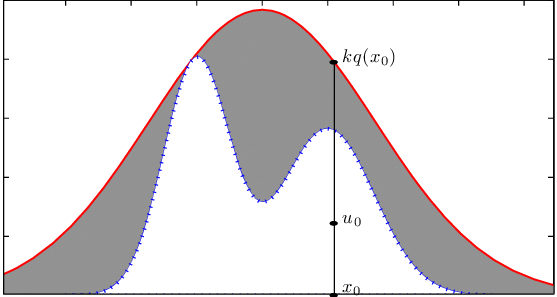
\includegraphics[width=0.3\textwidth]{figures/sampling_rejection_sampling.png}
		\caption{Visualizing rejection sampling. In the figure, $\tilde{q}(z)$ is denoted as $kq(z)$, and $x_0$ is the initial sample from $q$.}
		\label{fig:sampling_rejection_sampling}
	\end{figure}
	\item To show that we actually generate samples from $p(z)$, we can write down the probability for a value $z_i$ to be picked. First, the chance of $z_i$ being generated in first place is $q(z_i)$. Next, the chance of $z_i$ being accepted, is $\frac{\tilde{p}(z_i)}{\tilde{q}(z_i)}$. Together, we get the probability of $z_i$:
	$$\hat{p}(z_i) = q(z_i)\frac{\tilde{p}(z_i)}{\tilde{q}(z_i)} \propto p(z_i)$$
	Hence, we actually generate samples from $z_i$ although we initially sample from $q(z)$
	\item One requirement of rejection sampling to work well is that the area between $\tilde{p}(z)$ and $\tilde{q}(z)$ is small. The efficience of this sampler can be measured by the acceptance rate, which is $\E_{z_i\sim q}\left[\frac{\tilde{p}(z_i)}{\tilde{q}(z_i)} \right]$. If this value is low, it means that a lot of samples are rejected, hence the sampling process takes longer. This gets especially critical in higher dimensions as we need to make sure that \textit{for all} $z_i$, $\tilde{q}(z_i)$ is greater than $\tilde{p}(z_i)$. Finding a simple distribution in high dimensions that fulfills this requirement is often not trivial
\end{itemize}
\subsection{Importance sampling}
\begin{itemize}
	\item Another approach for estimating an expectation is not generating actual samples from $p$, but simply weight samples by their \textit{importance}
	\item Again, we need two distributions: $p$ over which we want to determine the expectation, and $q$ that we actually sample from. Note that for this algorithm to work, none of these distributions need to be normalized. The only thing that is required is that we can sample from the normalized density of $q$.
	\item The pseudo-code for the importance sampling is fairly simple and straight forward: \begin{tcolorbox}[colback=white!85!gray,colframe=gray!75!black,title=Pseudocode for importance sampling]
		\begin{algorithm}[H]
			\SetAlgoLined
			Sample $\left\{z_n\right\}_{n=1}^{N}$ from $q(z)$\;
			Calculate the weights $w_n=\frac{p(z_n)}{q(z_n)}$\;
			Determine expectation by $\E_p[f]\approx \frac{\sum_n w_n f(z_n)}{
			\sum_n w_n}$\;
		\end{algorithm}
	\end{tcolorbox}
	\item The intuition of importance sampling can be shown when plugging in the two distributions:
	$$\E_p[f]=\int p(z)f(z)dz=\frac{\int q(z)\frac{p(z)}{q(z)}f(z)dz}{\underbrace{\int q(z)\frac{p(z)}{q(z)}dz}_{=1}} = \frac{\E_q\left[w_z\cdot f(z)\right]}{\E_q\left[w_z\right]} \approx \E_q\left[\frac{\sum_i w_i f(z_i)}{\sum_i w_i}\right]$$
	\item Although importance sampling can use all samples, it has two major drawbacks:
	\begin{itemize}
		\item The estimate of $\E[f]$ is \underline{not} unbiased. Imagine we would sample only a single time ($N=1$ in pseudo code). As the sum drops out, we end up with $f(z_i)$ where $z_i$ is sampled from $q$, and not $p$! This bias decreases with the number of samples, but should always be kept in mind as an accurate estimate might require more samples, especially when it occurs with the second drawback.
		\item The importance weighting estimate has a high variance if $p$ differs strongly from $q$, especially when $p(z_i)\gg q(z_i)$ as the weight is very high for this data point. Imagine $q$ is a Gaussian with a large variance, while $p$ is a peaked Gaussian around 0. For most of the samples, $p(z)\ll q(z)$, and hence their weight is low. But for a small set of points, namely those close to 0, $p(z)$ is much greater than $q(z)$ resulting in a high weight. If we now sample e.g. 100 times, all points except those around 0 are neglected due to their low weight. And as those important points are rarely sampled from $q$, we need many samples to reduce the variance. This problem occurs even stronger in high-dimensional spaces.
	\end{itemize}
	\item Furthermore, note that importance sampling can only be used for approximating an expectation, and not for generating independent samples from $p$
\end{itemize}
\subsection{Ancestral Sampling}
\begin{itemize}
	\item Assume we have given a Bayesian network, and want to sample from the joint probability. We can write the joint probability as:
	$$p(\bm{z})=\prod_{i=1}^{d} p(z_i\vert z_{\text{pa}(i)})$$
	where we use a topological ordering $z_1,...,z_d$ with $z_j<z_i$ if $j\in \text{pa}(i)$
	\item Now we can simply sample from the joint distribution by sampling from each of the conditionals, in the topological ordering. For example, assume we have the following Bayesian network:
	
	\begin{figure}[ht!]
		\centering
		\tikz{ %
			\node[latent] (z1) {$z_1$} ; %
			\node[latent, right=of z1] (z3) {$z_3$} ; %
			\node[latent, above=of z3] (z2) {$z_2$} ; %
			\node[latent, below=of z3] (z4) {$z_4$} ; %
			\node[latent, right=of z2] (z5) {$z_5$} ; %
			\node[latent, right=of z4] (z6) {$z_6$} ; %
			
			\edge{z1}{z2};
			\edge{z1}{z3};
			\edge{z1}{z4};
			\edge{z2}{z5};
			\edge{z3}{z5};
			\edge{z3}{z6};
			\edge{z2}{z6};
			\edge{z4}{z6};
		}
	\end{figure}

	Then we can sample as follows:
	\begin{equation*}
		\begin{split}
			\tilde{z}_1 & \sim p(z_1)\\
			\tilde{z}_2 & \sim p(z_2|z_1=\tilde{z}_1)\\
			\tilde{z}_3 & \sim p(z_3|z_1=\tilde{z}_1)\\
			\tilde{z}_4 & \sim p(z_4|z_1=\tilde{z}_1)\\
			\tilde{z}_5 & \sim p(z_5|z_2=\tilde{z}_2,z_3=\tilde{z}_3)\\
			\tilde{z}_6 & \sim p(z_6|z_2=\tilde{z}_2,z_3=\tilde{z}_3,z_4=\tilde{z}_4)\\
		\end{split}
	\end{equation*}
	
	\item Note that for sampling from each of the individual distributions, we can use the other techniques like rejection or importance sampling. 
	
	% \item \TODO{Question: lecture notes say that it works badly with high dimensions, but other sources say it works well. Why would it not work in high dimensions?}
\end{itemize}
\subsection{Markov-Chain Monte Carlo}
\begin{itemize}
	\item Given a target distribution $p(x)$ that we want to sample from, we setup a Markov chain such that $p(x_n)\to p(x)$ as $N\to\infty$, i.e. such that $p(x)$ is its equilibrium distribution
	
	\begin{figure}[ht!]
		\centering
		\tikz{ %
			\node[latent] (x1) {$x_1$} ; %
			\node[latent, right=of x1] (x2) {$x_2$} ; %
			\node[latent, right=of x2] (x3) {$x_3$} ; %
			\node[const, right=of x3] (xetc1) { \hspace{2mm}...\hspace{2mm} } ; %
			\node[latent, right=of xetc1] (xN) {$x_N$} ; %
			\node[const, right=of xN] (xetc2) { \hspace{2mm}...\hspace{2mm} } ; %
			\node[latent, right=of xetc2] (xInfty) {$x_{\infty}$} ; %
			
			\edge{x1}{x2};
			\edge{x2}{x3};
			\edge{x3}{xetc1};
			\edge{xetc1}{xN};
			\edge{xN}{xetc2};
			\edge{xetc2}{xInfty};
		}
	\end{figure}
	\item Note that as MCMC runs ancestral sampling on a chain, two consecutive samples are no longer independent. Still, we can assume that the dependency between two fairly distant samples is neglectable
	\item We start sampling $x_1$ from an initial distribution $q(x_1)$ which can be chosen arbitrarily (but the closer $q$ to $p$, the faster the convergence and hence, faster sampling). For the next samples, we use a \underline{transition kernel} $T$ (which we have to specify/find by ourselves) to get $x_2\sim T(x_2|x_1)$
	\item The transition kernel is usually independent of time (most efficient), but can be extended to multiple steps (e.g. $x_t$ is sampled by $T_1$, $x_{t+1}$ from $T_2$, and $x_{t+2}$ again from $T_1$)
	\item The marginal distribution can be determined by:
	$$q(x_{n}) = \int q(x_{n-1})T(x_{n}|x_{n-1})dx_{n-1}$$
	and the joint probability for all $x_1,...,x_N$ is:
	$$q(x_1,...,x_N) = q(x_1)\prod_{i=2}^{N}T(x_i|x_{i-1})$$
	\item The equilibrium is reached when $x_N\sim p(x)$ (i.e. $p(x)$ is an invariant of the chain):
	$$p(x_{N+1}) = \int T(x_{N+1}|x_N)p(x_N)dx_N$$ 
	In this case, $p(x)$ is called to be an invariant of the chain. Note that a chain can have multiple invariants, as if $T$ is the identity transformation, any distribution is an invariant of that chain
	\item A sufficient but not necessary condition of an invariant $p(x)$ is that it satisfies the property of \underline{detailed balance}:
	$$p(x_t)T(x_{t+1}|x_t) = p(x_{t+1})T(x_t|x_{t+1})$$
	This property can be interpreted as the Markov chain being reversible. Although detailed balance is not required, it is mostly easier to fulfill when designing a kernel
	\item Another property we are looking for is \underline{ergodicity}. A sufficient condition for ergodicity is that any state $x_N$ has a positive probability, for any $N$.
	\item If we have an ergodic Markov chain and $p^{\star}(x)$ being an invariant, then $p^{\star}(x)$ is a unique equilibrium, where for any start distribution $q(x_0)$, the distribution $q(x_N)$ with $N\to\infty$ converges to the required distribution $p^{\star}(x)$.
	\item The sketch of the sampling process is:
	
	\begin{algorithm}[H]
		Sample initial state $x_0$ from $q(x_0)$\;
		\For{$t=0,...,N$}{
			Sample $x_{t+1}\sim T(x_{t+1}|x_{t})$\;
		}
		Output $x_N$ as sample of $p^{\star}(x)$\;
	\end{algorithm}
	$N$ has to be large enough in this case, and is often referred to as \textit{burn-in} time. 
	
	In addition, note that the required $N$ can be reduced by reducing the distance between $q$ and $p$. Thus, for generating multiple samples, we can take the first sample $x_N$, and continue the chain for additional $M$ steps, where usually $M\ll N$ (but $M$ must be certain size to guarantee independence of samples, depends on $T$). Then, $x_{N+M}$ is a new sample from $p$.
	
	\item The problem of MCMC is how we can find the transition kernel $T$ for a distribution $p$. Once we have found two kernels, we can combine those to new kernels:
	\begin{equation*}
		\begin{split}
			T_3 & = \alpha T_1 + (1 - \alpha) T_2, \hspace{2mm}(\alpha \in [0,1])\\
			T_3 & = T_2 \circ T_1 \hspace{5mm}(\text{composition, first apply $T_1$, then $T_2$})
		\end{split}
	\end{equation*}
	\item One way to overcome this problem is the Metropolis-Hastings algorithm, which uses a form of rejection sampling to allow any transition kernel $T$
\end{itemize}
\subsubsection{Metropolis-Hastings algorithm}
\begin{itemize}
	\item Choose a proposal transition kernel $Q(x_{t+1}|x_{t})$ (e.g. a random walk). Then we can sample from $p^{\star}(x)$ as follows:
	\begin{tcolorbox}[colback=white!85!gray,colframe=gray!75!black,title=Pseudocode for Metropolis-Hastings algorithm]
		\begin{algorithm}[H]
			\SetAlgoLined
			Sample initial state $x_0$ from $q(x_0)$\;
			\For{$t=0,...,N$}{
				Sample $\tilde{x}_{t+1}\sim Q(\tilde{x}_{t+1}|x_{t})$\;
				Compute acceptance probability $\alpha(\tilde{x}_{t+1}|x_t) = \min\left(1, \frac{p^{\star}(\tilde{x}_{t+1}) Q(x_t|\tilde{x}_{t+1})}{p^{\star}(x_t)Q(\tilde{x}_{t+1}|x_{t})}\right)$\;
				Sample $u_t\sim U(0,1)$\;
				\eIf{$u_t \leq \alpha(\tilde{x}_{t+1}|x_t) $}{accept sample $x_{t+1}=\tilde{x}_{t+1}$\;}{reject sample and stay at current state: $x_{t+1}=x_t$\;}
			}
			Output $x_N$ as sample of $p^{\star}(x)$\;
		\end{algorithm}
	\end{tcolorbox}	
	We can view the combination of $Q$ and acceptance probability $\alpha$ as our transition kernel $T=\alpha\circ Q$.
	\item Given this simple algorithm, we can design the transition kernel $Q$ with minimal knowledge of $p^{\star}$. For example, a kernel which mostly works well is to combine larger and smaller random walk steps. This can be very helpful in high-dimensional space as it can explore in different scales, and hence, in contrast to rejection and importance sampling, still works well in high dimensions
	\item Nonetheless, keep in mind that the performance now depends on the transition kernel $Q$. If it is designed poorly, many samples are rejected and we again end up with an inefficient sampling process. For example, if we have a highly multi-modal distribution, we need to have large enough steps to be able to jump between modes. But as said before, this is much less knowledge we need of $p^{\star}$ compared to the other discussed sampling algorithms
	\item We can sketch the proof here for the detailed balance. If a new sample $x_{t+1}$ is accepted, it has the probability:
	\begin{equation*}
		\begin{split}
			p^{\star}(x_t)T(x_{t+1}|x_{t}) & = p^{\star}(x_t)Q(x_{t+1}|x_{t})\min\left(1, \frac{p^{\star}(x_{t+1}) Q(x_t|x_{t+1})}{p^{\star}(x_t)Q(x_{t+1}|x_{t})}\right)\\
			& = \min\left(p^{\star}(x_t)Q(x_{t+1}|x_{t}), p^{\star}(x_{t+1}) Q(x_t|x_{t+1})\right)\\
			& = p^{\star}(x_{t+1})Q(x_{t}|x_{t+1})\min\left(1, \frac{p^{\star}(x_{t}) Q(x_{t+1}|x_{t})}{p^{\star}(x_{t+1})Q(x_{t}|x_{t+1})}\right)\\
			& = p^{\star}(x_{t+1})T(x_{t}|x_{t+1})
		\end{split}
	\end{equation*}
	As we can interchange $x_t$ and $x_{t+1}$, $p^{\star}$ is an invariant of the Markov chain.
	
	In case $\tilde{x}_{t+1}$ was rejected, we stay at $x_t$ which satisfies the detailed balance anyways.
\end{itemize}
\subsubsection{Gibbs sampling}
\begin{itemize}
	\item Gibbs sampling is a special case of the Metropolis-Hastings algorithm, where the acceptance probability is always 1. The idea is that we cannot easily sample from a big joint distribution, but sampling a single variable given all others is feasible/much simpler. 
	\item Hence, we sample a D-dimensional vector $(x_1,x_2,...,x_D)$ by sampling from the conditional distributions of a single variable $x_i$ where we keep all other variables fixed. In pseudo-code, we can define Gibbs sampling as:
	\begin{tcolorbox}[colback=white!85!gray,colframe=gray!75!black,title=Pseudocode for Gibbs sampling]
		\begin{algorithm}[H]
			\SetAlgoLined
			Choose an initial state $\left\{x_i:i=1,...,M\right\}$\;
			\For{$t=0,...,N$}{
				Sample $x_1^{(t+1)}\sim p(x_1|x_2^{(t)}, x_3^{(t)},...,x_M^{(t)})$\;
				Sample $x_2^{(t+1)}\sim p(x_2|x_1^{(t+1)}, x_3^{(t)},...,x_M^{(t)})$\;
				... \\
				Sample $x_M^{(t+1)}\sim p(x_M|x_2^{(t+1)}, x_3^{(t+1)},...,x_{M-1}^{(t+1)})$\;
			}
			Output $\left\{x_1^{(N)},...,x_M^{(N)}\right\}$ as sample of $p(x_1,...,x_M)$\;
		\end{algorithm}
	\end{tcolorbox}	
	\item Clearly, $p(\bm{x})$ is an invariant of the Markov chain because at each step, we sample from the correct conditional $p(x_i,\bm{x}_{\setminus i})$. But note that detailed balance can only be guaranteed if the order of $x_i$'s is randomized every iteration.
	\item For ergodicity, we just need to make sure that the conditionals are not zero for any point. Otherwise, we have to prove ergodicity explicitly.
	\item The acceptance probability of a sample according to the Metropolis-Hastings algorithm is in case of Gibbs sampling:
	$$\alpha(\bm{x}^{(t+1)}|\bm{x}^{(t)}) = \frac{p^{\star}(\bm{x}^{(t+1)}) Q(\bm{x}^{(t)}|\bm{x}^{(t+1)})}{p^{\star}(\bm{x}^{(t)})Q(\bm{x}^{(t+1)}|\bm{x}^{(t)})} = \frac{p^{\star}(x_i^{(t+1)}|\bm{x}_{\setminus i}^{(t+1)})p^{\star}(\bm{x}_{\setminus i}^{(t+1)})\cdot p^{\star}(x_i^{(t)}|\bm{x}_{\setminus i}^{(t+1)})}{p^{\star}(x_i^{(t)}|\bm{x}_{\setminus i}^{(t)})p^{\star}(\bm{x}_{\setminus i}^{(t)})\cdot p^{\star}(x_i^{(t+1)}|\bm{x}_{\setminus i}^{(t)})} = 1$$
	where $\bm{x}_{\setminus i}^{(t)}=\bm{x}_{\setminus i}^{(t+1)}$ as the other variables do not change.
\end{itemize}